\section{Introduction to Lattice}

\begin{defBox}{Lattice}
    aA lattice $\mathcal{L}$ is a discrete subgroup of $\mathbb{R}^n$.
\end{defBox}

\noindent
Discrete means that, given an element of $\mathcal{L}$, there exists a neighborhood of such element that contains no other elements of $\mathcal{L}$. So, we can isolate our elemtns of the lattice.

\begin{figure}[h!]
  \centering
  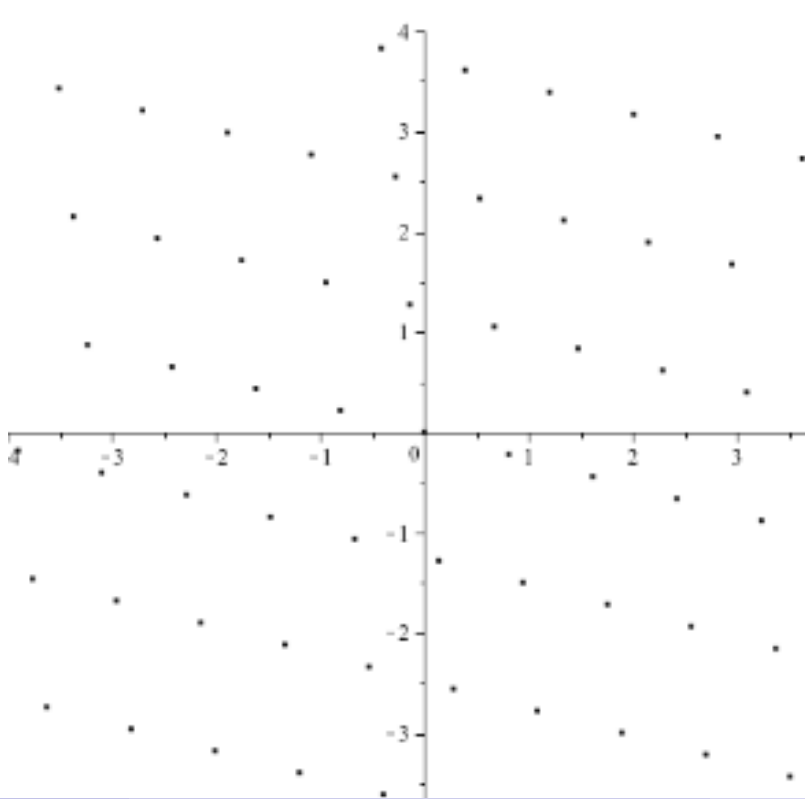
\includegraphics[width=0.5\textwidth]{images/section_6/lattice.png}
  \caption{Lattice in $\mathbb{R}^2$}
  \label{fig:lattice}
\end{figure}

\begin{defBox}{Rank}
    tThe rank of a lattice $\mathcal{L} \subset \mathbb{R}^n$, $rk(\mathcal{L})$ is the maximum number of linearly independent vectors in $\mathcal{L}$.\\
    The lattice is called \textbf{full-rank} or \textbf{complete} if rk($\mathcal{L}$) = $n$.\\
    If $\mathcal{L} \subset \mathbb{Z}^n$ is called \textbf{integer lattice}.
\end{defBox}

\noindent
\textbf{Example}
\begin{itemize}
    \item $\mathbb{Z}^5$  is a lattice
    \item $\{(x, 2x): x \in \mathbb{Z}\}$ is a lattice
    \item $\{(x, 2x): x \in \mathbb{R}\}$ is not a lattice, because it is not discrete.
    \item $\{(2x, x+1): x \in \mathbb{Z}\}$ is not a lattice, because it is not a subgroup of $\mathbb{R}^2$.
\end{itemize}

\subsection{Some properties of lattices}
The intersection of two lattices is a lattice of $\mathbb{R}^n$ is a lattice in $\mathbb{R}^n$.
\medskip

\noindent
If $\mathcal{L}$ is a lattice in $ c \in \mathbb{R}^x$ then
\begin{center}
    $\mathcal{L}c = \{cv: v \in \mathcal{L}\}$ is a lattice in $\mathbb{R}^n$.
\end{center}
This means that we procude a set by multiplying all elements of the lattice by a constant $c$
\medskip

\noindent
If $\mathcal{L}_1$ and $\mathcal{L}_2$ are lattices in $\mathbb{R}^n$ then
\begin{center}
    $\mathcal{L}_1 + \mathcal{L}_2 = \{v_1 + v_2: v_1 \in \mathcal{L}_1, v_2 \in \mathcal{L}_2\}$ is not in general a lattice in $\mathbb{R}^n$.
\end{center}
That because we can lost the discreteness property.
\bigskip

\begin{defBox}{Minimum Distance}
    GGiven a lattice $\mathcal{L}$, we define the minimum distance of $\mathcal{L}$, denoted by $\lambda(\mathcal{L})$, as the length of the shortest non-zero vector in $\mathcal{L}$
    \begin{center}
        $\lambda(\mathcal{L}) = \min\{\|v\|: v \in \mathcal{L} \setminus \{0\}\}$
    \end{center}
\end{defBox}
\noindent
Let us observe that $\lambda(\mathcal{L}) = \min\{\|v\|: v \in \mathcal{L} \setminus \{0\}\} = \min \{\|v - w\|: v, w \in \mathcal{L}, v \neq w\}$
\bigskip 

\noindent
A lattice $\mathcal{L}$ of $\mathbb{R}^n$ is generated by a finite number of linearly independent vectors.

\begin{defBox}{Basis}
    AA basis $\mathcal{B}$ of a lattice $\mathcal{L}$ is a set of linearly independent generators of $\mathcal{L}$.\\
    If $\mathcal{B} = \{b_1, b_2, \ldots, b_k\}$, then 
    \begin{center}
        $\mathcal{L} = \{\sum_{i=1}^k z_i b_i: z_i \in \mathbb{Z}\}$
    \end{center}
    where $k$ is the rank of $\mathcal{L}$.
\end{defBox}

\noindent
Each lattice can has many different bases.
\medskip

\noindent
A basis can be rapresented by a $r \times n$ matrix
\begin{center}
    $B = \begin{bmatrix}
    b_{1}\\
    b_{2}\\
    \vdots\\
    b_{r}
    \end{bmatrix}$
\end{center}
so that $\mathcal{L} = \{aB: a \in \mathbb{Z}^r\}$, where $a$ is a row vector of $\mathbb{Z}^r$.
\medskip

\noindent
If $B_1$ and $B_2$ are two bases of the same lattice $\mathcal{L}$, then there exists a unimodular matrix $U$ such that $B_1 = UB_2$.\\
\bigskip

\noindent
NOT EVERY set of r linearly independent vectors in a lattice is a basis.\\
This is true if the ”parallelepiped” it determines does not contain any point of $\mathcal{L}$ except its vertices.
\medskip

\noindent
A lattice can have a proper sublattice of the same rank.
\medskip

\noindent
A lattice does not admit in general an orthogonal basis

\subsubsection{Foundamental Domain}

\begin{defBox}{Foundamental Domain}
    LLet $\mathcal{L}$ be a lattice of rank $n$  with basis $\mathcal{B} = \{b_1, b_2, \ldots, b_n\}$. \\
    The foundamental domain is 
    \begin{center}
        $\mathcal{F}(\mathcal{B}) = \{\sum_{i=1}^n \alpha_i b_i: 0 \leq \alpha_i < 1\}$
    \end{center}
\end{defBox}

\begin{defBox}{Determinant}
    aGiven any basis $B$ (in matricial form) of a lattice $\mathcal{L}$, the determinant of $\mathcal{L}$, denoted det($\mathcal{L}$), is the volume of the fundamental domain. If $\mathcal{L}$ is full rank, then det($\mathcal{L}$) = $|\det B|$.
\end{defBox}

\noindent
\textbf{Remark:} The determinant is an invariant, i.e., it does not depend on the choice of the basis.
\medskip



\noindent
\textbf{Example:}\\
Consider the lattice generated by vectors $b_1 = (2, 1)$ and $b_2 = (1, -1)$, then the foundamental domain is the parallelogram determined by $b_1$ and $b_2$. [see Figure \ref{fig:foundamental_domain}]

\begin{figure}[h!]
  \centering
  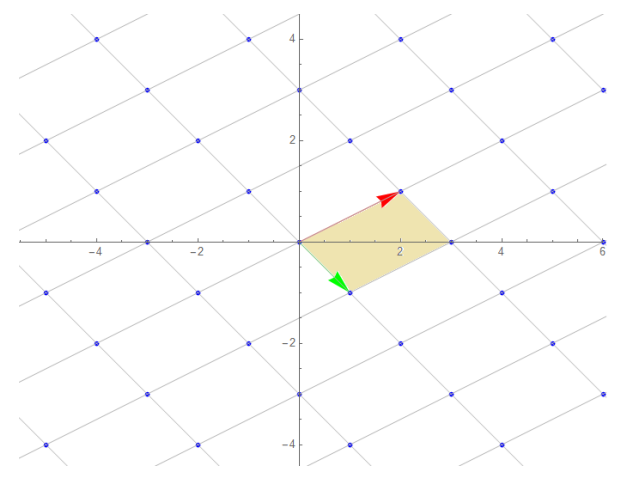
\includegraphics[width=0.75\textwidth]{images/section_6/foundamental_domain_1.png}
  \caption{Foundamental Domain}
  \label{fig:foundamental_domain}
\end{figure}

\noindent
Lattice generated by the vectors $b_1 = (1, 0, 0)$, $b_2 = (0, 1, 0)$ and $b_3 = (0, 0, 1)$ the foundamental domain is the cube determined by $b_1$, $b_2$ and $b_3$. [see Figure \ref{fig:foundamental_domain_cube}]

\begin{figure}[h!]
  \centering
  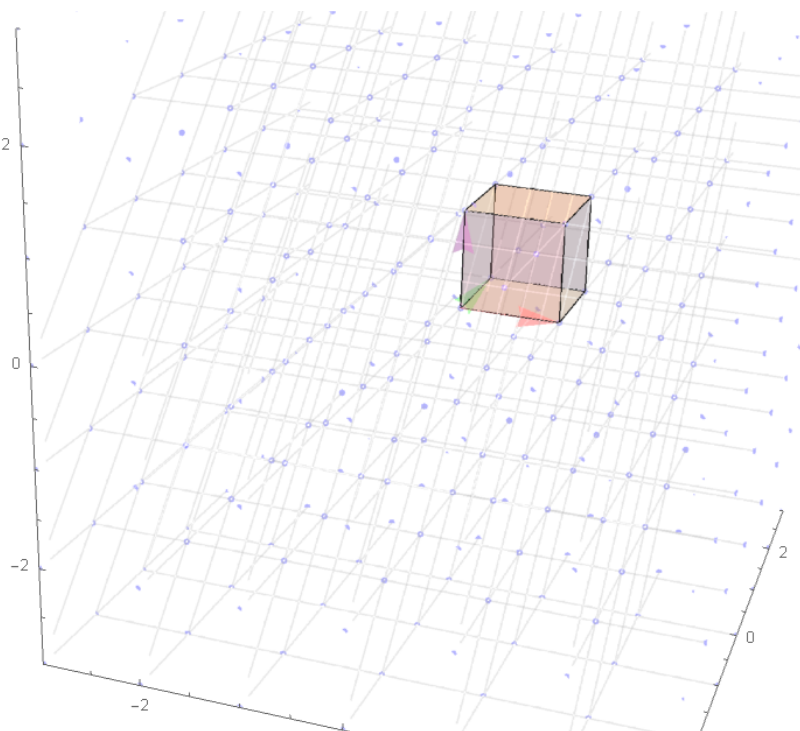
\includegraphics[width=0.75\textwidth]{images/section_6/foundamental_domain_3.png}
  \caption{Foundamental Domain in $\mathbb{R}^3$}
  \label{fig:foundamental_domain_cube}
\end{figure}

\newpage
\begin{propBox}{Minkowski's Bound}{}
    How long is a shortest nonzero vector in a lattice $\mathcal{L}$ of $\mathbb{R}^n$? The lattice $\mathcal{L}$ contains a nonzero vector $v$ satisfying:
    \begin{center}
        $\|v\| \leq \sqrt{n} \cdot (\det(\mathcal{L}))^{1/n}$
    \end{center}
\end{propBox}

\medskip

\begin{propBox}{}{}
    Let $\mathcal{L} \subset \mathbb{R}^n$ be a lattice of rank $n$, then $\forall v \in \mathbb{R}^n$ we have 
    \begin{center}
        $v = b + f$
    \end{center}
    for a unique $b \in \mathcal{L}$ and a unique $f \in \mathcal{F}$
\end{propBox}
\noindent
It is possible to provide a one-to-one correspondence between lattice and polynomials by means of the following mapping:
\begin{align*}
    \mathbb{Z}^n &\leftrightarrow \mathbb{Z}[x]_{< n}, (a_0, a_1, \ldots, a_{n-1}) \leftrightarrow a_0 + a_1 x + \ldots + a_{n-1} x^{n-1}
\end{align*}

\noindent
An ideal lattice is a lattice $\mathcal{L} \subseteq \mathbb{Z}^n$ such that is isomorphic to an ideal $I \subseteq \mathbb{Z}_{[X]}/(f(x))$ with $f(x) \in \mathbb{Z}[x]$ monic and irreducible polynomial


\subsection{Lattice Problems}
We are interested to define some computational problems related to lattices, that are the basis of the security of lattice-based cryptography.

\begin{defBox}{Shortest Vector Problem (SVP)}
    aGiven a lattice $\mathcal{L} \subseteq \mathbb{Z}^n$.\\
    The Shortest Vector Problem (SVP) is the problem of finding a non-zero vector $v \in \mathcal{L}$ such that $\|v\|= \min_{x \in \mathcal{L}, x \neq 0} \|v\| = \lambda(\mathcal{L})$. 
\end{defBox}

\begin{figure}[h!]
  \centering
  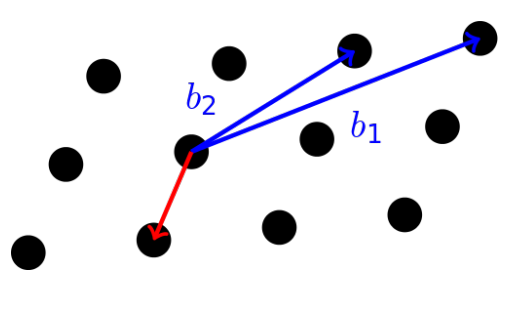
\includegraphics[width=0.4\textwidth]{images/section_6/SVP.png}
  \caption{Shortest Vector Problem}
  \label{fig:SVP}
\end{figure}

\begin{defBox}{Approximated SVP problem (SVP-$\gamma$)}
    TThe approximated SVP problem (SVP-$\gamma$) is the problem of finding a vector $v \in \mathcal{L}$ such that $\forall x \in \mathcal{L}$:
    \begin{center}
        $\|v \| \leq \gamma \min\|x\|$
    \end{center}
    where $\gamma \geq 1$ is an approximation factor.
\end{defBox}

\begin{defBox}{Closest Vector Problem (CVP)}
    gGiven a lattice $\mathcal{L} \subseteq \mathbb{Z}^n$ and a target vector $w \in \mathbb{R}^n$.\\
    The Closest Vector Problem (CVP) is the problem of finding a vector $v \in \mathcal{L}$ such that
    \begin{align*}
        \|v - w\| = \min_{x \in \mathcal{L}} \|x - w\|
    \end{align*}
\end{defBox}
\begin{figure}[h!]
  \centering
  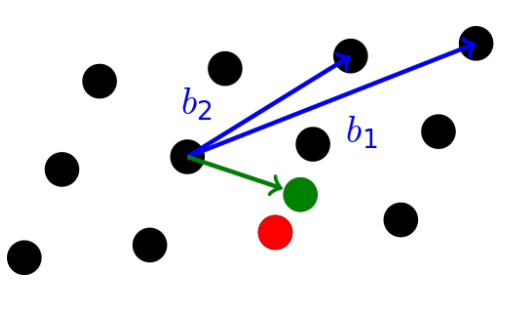
\includegraphics[width=0.4\textwidth]{images/section_6/CVP.png}
  \caption{Closest Vector Problem}
  \label{fig:CVP}
\end{figure}

\begin{defBox}{Approximated CVP problem (CVP-$\gamma$)}
    TThe approximated CVP problem (CVP-$\gamma$) is the problem of finding a vector $v \in \mathcal{L}$ such that $\forall x \in \mathcal{L}$:
    \begin{center}
        $\|v - w\| \leq \gamma \min\|x - w\|$
    \end{center}
    where $\gamma \geq 1$ is an approximation factor.
\end{defBox}

\noindent
SVP and CVP are computationally equivalent.\bigskip

\subsubsection*{Orthogonal basis case}
Both SVP and CVP are easy to solve if a lattice $\mathcal{L}$ of rank $n$ has an orthogonal basis $B = \{b_1, \ldots, b_n\}$ (considering a full rank lattice). Indeed, if $a_i \in \mathbb{Z}$, $t_i \in \mathbb{R}$ for all $i = 1, \ldots, n$ and $v \in \mathcal{L}$ we have:
\begin{align*}
    v &= \sum_{i=1}^n a_i b_i \implies \|v\|^2 = \sum_{i=1}^n a_i^2 \|b_i\|^2 \\
    w &= \sum_{i=1}^n t_i b_i \implies \|w - v\|^2 = \sum_{i=1}^n (a_i - t_i)^2 \|b_i\|^2
\end{align*}
Therefore to solve SVP we search the shortest nonzero vector in the set $\{\pm b_1, \ldots, \pm b_n\}$ and to solve CVP we take each $a_i$ as the integer closest to the corresponding $t_i$.


\subsubsection*{Lattices and Non-Orthogonal Bases}

Consider a lattice $L \subseteq \mathbb{R}^n$ of rank 2 whose basis is $\underline{b}_1 = (5, 1, 1)$ and $\underline{b}_2 = (4, 0, 1)$.
This is not an orthogonal basis, indeed:
\[ \underline{b}_1 \cdot \underline{b}_2 = 5 \cdot 4 + 1 \cdot 0 + 1 \cdot 1 = 21 \neq 0 \]

The lengths of these vectors are:
\[ ||\underline{b}_1|| = \sqrt{5^2 + 1^2 + 1^2} = \sqrt{27} \]
\[ ||\underline{b}_2|| = \sqrt{4^2 + 0^2 + 1^2} = \sqrt{17} \]

Let $\underline{v} = (v_1, v_2, \dots, v_n) \in \mathbb{R}^n$. Remember that the length of a vector is:
\[ ||\underline{v}|| = \sqrt{\underline{v} \cdot \underline{v}} = \sqrt{v_1^2 + v_2^2 + \dots + v_n^2} \]

\noindent
The shortest vector of $L$ is not, in this case, a vector of the basis. Indeed, for instance, $\underline{b}_1 - \underline{b}_2 \in L$ because it is a linear combination of $\underline{b}_1$ and $\underline{b}_2$ with integer coefficients. Since $\underline{b}_1 - \underline{b}_2 = (1, 1, 0)$, we have:
\[ ||\underline{b}_1 - \underline{b}_2|| = \sqrt{1^2 + 1^2 + 0^2} = \sqrt{2} \]
which is smaller than the length of $\underline{b}_1$ and $\underline{b}_2$.
\medskip

\noindent
Thus, in general, given a lattice $L$ and a non-orthogonal basis, the shortest vector is not necessarily a vector of the basis.

\subsubsection*{Lattices and Orthogonal Bases example}

Consider a lattice $L \subseteq \mathbb{R}^n$ of rank 2 whose basis is given by $\underline{b}_1$ and $\underline{b}_2$.\\ Suppose that this is an orthogonal basis, i.e., $\underline{b}_1 \cdot \underline{b}_2 = 0$.\\ 
Now, we see that the shortest vector of $L$ is a vector of the basis. 
\medskip

\noindent
A general vector $\underline{v}$ is a linear combination of $\underline{b}_1$ and $\underline{b}_2$ with integer coefficients: 
\[ \underline{v} = a_1\underline{b}_1 + a_2\underline{b}_2 \quad \text{with } a_1, a_2 \in \mathbb{Z} \]
\bigskip

\noindent
We consider the length of $\underline{v}$ squared (because it is more convenient):
\begin{align*}
||\underline{v}||^2 &= \underline{v} \cdot \underline{v} = (a_1\underline{b}_1 + a_2\underline{b}_2) \cdot (a_1\underline{b}_1 + a_2\underline{b}_2) \\
&= a_1^2(\underline{b}_1 \cdot \underline{b}_1) + a_2^2(\underline{b}_2 \cdot \underline{b}_2) + a_1a_2(\underline{b}_1 \cdot \underline{b}_2) + a_2a_1(\underline{b}_2 \cdot \underline{b}_1)
\end{align*}

\vspace{0.5cm}

\noindent
Since $a_1, a_2 \in \mathbb{Z}$ (and assuming $\underline{v} \neq \underline{0}$), we have $a_1^2 \ge 1$ or $a_2^2 \ge 1$, and consequently:
\[ ||\underline{v}||^2 \ge ||\underline{b}_1||^2 \quad \text{and} \quad ||\underline{v}||^2 \ge ||\underline{b}_2||^2 \]
Thus the shortest vector of $L$ can be $\underline{b}_1$ or $\underline{b}_2$.

\bigskip

\noindent
This holds in general. Consider $L \subseteq \mathbb{R}^n$ of rank $n$ with an orthogonal basis $\underline{b}_1, \dots, \underline{b}_n$.\\
For all $\underline{v} \in L$, we have $\underline{v} = a_1\underline{b}_1 + \dots + a_n\underline{b}_n$ with $a_i \in \mathbb{Z}$.

\begin{align*}
||\underline{v}||^2 &= \underline{v} \cdot \underline{v} = (a_1\underline{b}_1 + \dots + a_n\underline{b}_n) \cdot (a_1\underline{b}_1 + \dots + a_n\underline{b}_n) \\
&= a_1^2(\underline{b}_1 \cdot \underline{b}_1) + \dots + a_n^2(\underline{b}_n \cdot \underline{b}_n) = a_1^2||\underline{b}_1||^2 + \dots + a_n^2||\underline{b}_n||^2
\end{align*}

\noindent
Thus, if $L$ has an orthogonal basis, the shortest vector is a vector of the basis.

\subsubsection*{Closest Vector Problem}

A similar situation happens if, given $\underline{w} \in \mathbb{R}^n$, we search for the closest vector of $L$ to $\underline{w}$. In this case, we are searching for a vector $\underline{v} = a_1\underline{b}_1 + \dots + a_n\underline{b}_n \in L$ (with $a_i \in \mathbb{Z}$) that minimizes $||\underline{w} - \underline{v}||$, or equivalently $||\underline{w} - \underline{v}||^2$.
\medskip

\noindent
Since $\underline{b}_1, \dots, \underline{b}_n$ is a basis of $L$, it is also a basis of $\mathbb{R}^n$ (since they are linearly independent vectors), and:
\[ \underline{w} = t_1\underline{b}_1 + \dots + t_n\underline{b}_n \in \mathbb{R}^n \quad \text{with } t_i \in \mathbb{R} \]
\medskip

\noindent
We have $\underline{w} - \underline{v} = (t_1 - a_1)\underline{b}_1 + \dots + (t_n - a_n)\underline{b}_n$ and:

\begin{align*}
||\underline{w} - \underline{v}||^2 &= (\underline{w} - \underline{v}) \cdot (\underline{w} - \underline{v}) \\
&= \big((t_1 - a_1)\underline{b}_1 + \dots + (t_n - a_n)\underline{b}_n\big) \cdot \big((t_1 - a_1)\underline{b}_1 + \dots + (t_n - a_n)\underline{b}_n\big) \\
&= (t_1 - a_1)^2(\underline{b}_1 \cdot \underline{b}_1) + \dots + (t_n - a_n)^2(\underline{b}_n \cdot \underline{b}_n) \\
&= (t_1 - a_1)^2||\underline{b}_1||^2 + \dots + (t_n - a_n)^2||\underline{b}_n||^2
\end{align*}

\noindent
This quantity is minimized if and only if:
\begin{itemize}
    \item $a_1$ is the closest integer to $t_1$
    \item $a_2$ is the closest integer to $t_2$
    \item $\dots$
    \item $a_n$ is the closest integer to $t_n$
\end{itemize}

\subsubsection{Gram-Schmidt Orthogonalization}

Given a basis $\underline{v}_1, \dots, \underline{v}_n$ of $\mathbb{R}^n$, it transforms this into an orthogonal basis $\underline{u}_1, \dots, \underline{u}_n$ of $\mathbb{R}^n$:

\begin{align*}
\underline{u}_1 &= \underline{v}_1 \\
\underline{u}_2 &= \underline{v}_2 - \text{proj}_{\underline{u}_1}(\underline{v}_2)
\end{align*}

\noindent
Where $\text{proj}_{\underline{u}_1}(\underline{v}_2)$ is the orthogonal projection of $\underline{v}_2$ onto $\underline{u}_1$.
\bigskip

\noindent
Let us check that $\underline{u}_2$ is orthogonal to $\underline{u}_1$. Geometrically, this is the sum (the diagonal of the parallelogram) between the vectors $\underline{v}_2$ and $-\text{proj}_{\underline{u}_1}(\underline{v}_2)$.

\vspace{1 cm}

\noindent
If a lattice $\mathcal{L}$ has a basis $\mathcal{B} = \{b_1, \dots, b_n\}$ we searche for a good basis having shortest vector which are \textit{"as orthogonal as possible to each others"}.
\medskip

\noindent
We can not directly use the correspondig Gram-Schmidt basis $\mathcal{B}^*= \{b_1^{*}, \dots, b_n^{*}\}$: it is not a basis for $\mathcal{L}$, since the Gram-Schmidt process does not preserve the integrality of the coefficients.\\
However, $\mathcal{B}$ has a good property:
\begin{align*}
    det(\mathcal{L}) = \prod_{i=1}^n ||b_i^{*}||
\end{align*}

\noindent
(since the change of the basis matrix from $\mathcal{B}$ to $\mathcal{B}^*$ has determinat equal to 1) and we could use $\mathcal{B}^*$ in oreder to find a new basis for $\mathcal{L}$ as similar as possible to $\mathcal{B}^*$

\subsubsection{LLL algorithm}
In a lattice $\mathcal{L}$ of rank $n$ we have the \textbf{LLL algorithm} to reduce a basis $\mathcal{B} = \{v_1, \dots, v_n\}$ with associated Gram-Schmidt orthogonal basis $\mathcal{B}^* = \{v_1^{*}, \dots, v_n^{*}\}$ to a new basis with vectors as ortogonal as possible.\\
A basis is LLL-reduced if:

\begin{itemize}
    \item \textbf{Size condition}:
    \begin{align*}
    |\mu_{i,j}| = \frac{| v_i, v_j^{*} |}{||v_j^{*}||^2} \leq \frac{1}{2} \quad \text{for all } 1 \leq j < i \leq n 
    \end{align*}
    \item \textbf{Lovasz condition}:
    \begin{align*}
    ||v_i^{*}||^2 \geq \left(\frac{3}{4} - \mu_{i, j}^2\right) ||v_{i-1}^{*}||^2 \quad \text{for all } 2 \leq i \leq n
    \end{align*}
\end{itemize}

\begin{algorithm}
\caption{Lenstra--Lenstra--Lovász (LLL) Reduction Algorithm}
\begin{algorithmic}[1]

\Require Basis $\mathcal{B}=\{v_1,\dots,v_n\}$ of an $n$-dimensional lattice $L$
\Ensure LLL-reduced basis $\mathcal{B}_{LLL}=\{v_1,\dots,v_n\}$

\State $k \gets 2$
\State $v_1^* \gets v_1$

\While{$k \leq n$}

    \For{$j = k-1, k-2, \dots, 1$}
        \State $v_k \gets v_k - \lfloor \mu_{k,j} \rceil v_j$
        \Comment{Size Reduction}
    \EndFor

    \If{$\|v_k^*\|^2 \geq \left(\dfrac{3}{4} - \mu_{k,k-1}^2\right)\|v_{k-1}^*\|^2$}
        \State $k \gets k+1$
    \Else
        \State Swap $v_{k-1}$ and $v_k$
        \State $k \gets \max\{k-1,2\}$
        \Comment{Swap}
    \EndIf

\EndWhile

\State \Return $\mathcal{B}_{LLL}$

\end{algorithmic}
\end{algorithm}
\noindent
\textbf{Note:}
\[
\mu_{k,j} = \frac{\langle v_k, v_j^* \rangle}{\|v_j^*\|^2}
\]
where the vectors $v_1^*,\dots,v_k^*$ are computed using the Gram--Schmidt orthogonalization process.

\subsection{Learning With Errors -- LWE}

\begin{defBox}{Learning With Errors (LWE)}
 lLet $p$ be a prime and let $n \in \mathbb{N}^+$.\\
 Given a secret vector $s \in \mathbb{Z}_p^n$.\\
 The \textbf{LWE-distribution} $A_{s, \chi}$ is defined as:

 \begin{align*}
    A_{s, \chi} = \{(a, b) \in \mathbb{Z}_p^n \times \mathbb{Z}_p
 \end{align*}

\noindent
such that: 
\begin{itemize}
    \item $a$ is chosen uniformly at random from $\mathbb{Z}_p^n$ (vector of lenght a)
    \item $b$ is defined as:
    \begin{align*}
        b= s \cdot a + e \mod p = (\langle s, a \rangle + e) \mod p
    \end{align*}
    where $e$ is an error term chosen according to a distribution $\chi$ over $\mathbb{Z}_p$.\\
    So $b$ is a a scalar, dot product between $s$ and $a$ plus an error term
\end{itemize}
\end{defBox}
\medskip

\noindent
LWE are typcally hard problems. In particular:
\begin{itemize}
    \item \textbf{Search LWE:} The problem Search $LWE_{n, p, \chi, m}$ is to find $s \in \mathbb{Z}_p^n$ given $m$ pairs $(a, b) \in A_{s, \chi}$
    \item \textbf{Decision LWE:} The problem Decision $LWE_{n, p, \chi, m}$ is to say, given $m$ pairs $(a, b) \in A_{s, \chi}$ and $m$ pairs $(a, b)$ where $a$ if they belong to a LWE distribution with a same fixed $s$ or if they are randomly sampled from a uniform distribution in $\mathbb{Z}_p^n \times \mathbb{Z}_p$.
\end{itemize}
\noindent
The two problems are computationally equivalent.
\bigskip

\noindent
In cryptography, is more convinient to work with the Ring-LWE problem.

\begin{defBox}{Ring Learning With Errors (Ring-LWE)}
    lConsider a prime $p$ and $n \in \mathbb{N}^+$, define $R = \mathbb{Z}_p[X] / (X^n + 1)$.\\
    Let $s = s(X) \in R$ a fixed element called secret, wich is a polynomial of degree at most $n-1$ with coefficients in $\mathbb{Z}_p$.\\
    The \textbf{Ring-LWE distribution} $A_{s, \chi}$ is defined as:
    \begin{align*}        
        A_{s, \chi} = \{(a, b) \} \subseteq R \times R
    \end{align*}
    such that:
    \begin{itemize}
        \item $a = a(X)$ is chosen uniformly at random from $R$ 
        \item $b = b(X)$ is defined as:
            \begin{align*}
                b = (s \cdot a + e) \mod p
            \end{align*}
            where $e = e(X)$ is an error term chosen according to a distribution $\chi$ over $R$.
    \end{itemize}
\end{defBox}

\noindent
Also Ring-LWE is a hard problem:
\begin{itemize}
    \item \textbf{Search Ring-LWE:} The problem Search $RingLWE_{n, p, \chi, m}$ is to find $s \in R$ given $m$ pairs $(a, b) \in A_{s, \chi}$
    \item \textbf{Decision Ring-LWE:} The problem Decision $RingLWE_{n, p, \chi, m}$ is to say, given $m$ pairs $(a, b) \in A_{s, \chi}$ if they come from a Ring-LWE distribution with a same fixed $s$ or if they are randomly sampled from a uniform distribution in $R \times R$.
\end{itemize}